\section{System Realization}
\label{sec:implementation}

\subsection{Typed model and executable profile}

\systemname{} realizes the contract with a typed object model.  Its
requirements, use-case, function, and verification concepts reuse a selected
EAST-ADL 2.1.12 foundation \cite{eastadl2013spec}; the \systemname{} namespace
adds scenario flow, entities, embodied agents, capabilities, runtime
bindings/actions, assertions, spatial responsibility, and handoffs.  EAST-ADL
is an implementation substrate for traceability, not the novelty claim, and we
do not claim full standard conformance.

Validation is deliberately staged.  A JSON schema checks required fields,
types, enumerations, and reference shapes.  The canonical V2 model checks
referential closure, typed cardinalities, unique source identifiers, assertion
ownership, and the absence of a direct step-to-action shortcut.  The executable
pipeline profile tightens compatibility cardinalities where runtime execution
needs one decision: a capability use requires one provider and capability, its
provider must agree with the performing agent and target responsibility, and a
published action must have a complete binding.  Runtime checks then bind one
specific request and response to an already valid, pinned instance.  Keeping
these stages separate identifies whether a failure belongs to serialization,
language well-formedness, the executable profile, or one runtime observation.

A room model stores stable \texttt{id} and \texttt{sourceId} values rather than
using labels or Unity GameObject names as identity.  Agents additionally have a
unique source-agent identifier and typed references to grounded assets, object
groups, responsible zones, provided capabilities, and handoff targets.
Runtime bindings own ordered actions with a locator and optional input/output
schemas.  A generated runtime projection contains only the data needed for
execution, while the canonical instance remains the source of truth.

\subsection{Generation and publication}

The project pipeline starts from structured room data and frozen semantic
artifacts.  It normalizes entities, associates objects with groups and zones,
derives agent roles and handoffs, materializes local knowledge, computes
placement, and assembles scenarios and capability uses.  Deterministic stages
create stable identifiers, runtime bindings, assertions, validation cases, a
trace map, and the backend runtime context.  Validators run before an atomic
publication step.  Content hashes record the model and dependent projections so
that stale outputs are detectable.

Language models can propose scene semantics, role labels, handoffs, and
knowledge during generation.  They do not choose runtime identifiers, decide
benchmark routes, or waive structural validation.  The frozen evaluation
corpus is subsequently regenerated and tested without a network or model API.

\subsection{Unity target binding and interaction state}

The Unity client imports the materialized room, agent configuration, model
projection, and trace map.  A scene-object component binds each relevant
collider to an exact model entity and source identifier.  Scene bootstrap
constructs a registry and fails on duplicate entities, duplicate source
matches, conflicting manual bindings, or missing target-specific contexts.
UUID-like suffixes are not accepted as approximate fallback identifiers.

In the evaluated desktop path, a camera ray selects a registered collider.  The
client retains the selection while the request is composed and represents
\texttt{none}, \texttt{resolved}, and \texttt{ambiguous} as distinct states.
A deictic request includes the pinned model hash, entity and source identifiers,
candidate identifiers, hit position, distance, selection modality, active
agent, and utterance.  Numeric ranges, list sizes, and string lengths are
bounded.  A missing or ambiguous selection is blocked before serialization.
The backend remains authoritative even when Unity performs the same earlier
check.

Figure~\ref{fig:unity-selection} shows the implemented Game view used in the
Steinpilz case.  The selected source object \texttt{brand\_panel3} is bound to
\texttt{ENT-ASSET-BRAND\_PANEL3}; the figure is evidence of the desktop
interaction path, not a headset study or a polished diagnostic interface.

\begin{figure}[t]
  \centering
  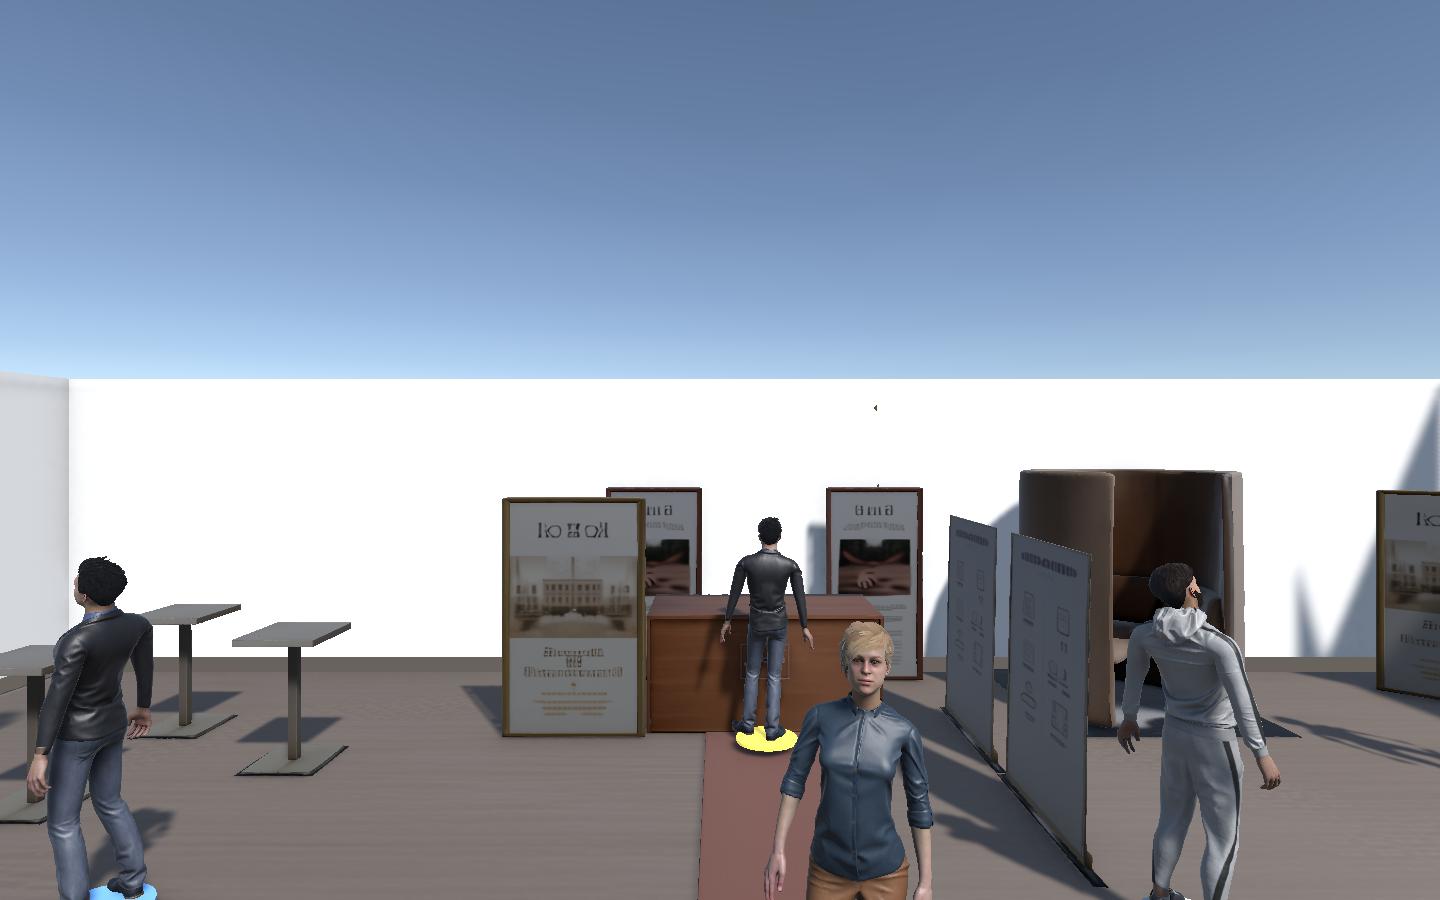
\includegraphics[alt={Unity Game view with a selected product panel and embodied agents},width=\columnwidth]{../paper/figures/unity-model-grounded-selection.png}
  \caption{Implemented Unity desktop view after loading the model-grounded
  scene and selecting \texttt{brand\_panel3}.  Runtime admission uses the
  stable entity binding rather than the visible label.}
  \Description{A Unity Game view of a virtual exhibition room with embodied
  agents and product panels.  One panel is selected and annotated with its
  stable source and model entity identifiers.}
  \label{fig:unity-selection}
\end{figure}

The multi-scenario bridge does not dispatch solely by an operation kind such as
``chat.''  It first uses the selected entity and server-resolved provider to
identify a candidate scenario context.  It accepts the scenario, capability,
binding, and action identifiers confirmed in the response and forwards the
event to the corresponding runner.  Zero or multiple exact contexts fail
closed.

\subsection{Authoritative backend admission}

Session setup loads the project contract, validates the native V2 instance and
trace map, builds a runtime context, and pins the model hash and contract
fingerprint to the session.  A changed project cannot be adopted silently:
preflight compares the current files with the pinned values and requires a new
setup after regeneration.

For each deictic chat request, the backend validates the spatial payload
strictly.  Unknown fields, non-finite or out-of-range ray values, excessive
candidate lists, conflicting entity and source identifiers, unknown objects,
non-scene entities, stale hashes, and ambiguous states are rejected.  The
backend derives the selected asset's group and zone from the runtime context;
it does not trust client-supplied ownership fields.

Responsibility resolution applies the asset--group--zone precedence and
identifies the source agent's permitted handoff edges.  The current request may
be answered locally or use one direct declared handoff.  Even when a provider
is graph-reachable through several agents, the online request is rejected
because one turn does not traverse a transitive path.  A later turn can start
from the active agent returned by the preceding accepted handoff and is checked
again under the same pinned contract.

The backend then selects an exact runtime action using the trusted scenario,
provider, and target.  A generic endpoint or action-kind match is insufficient.
Before generation, it snapshots the mutable session state.  If a
request-decidable check fails, the response model has not been called.  If the
structured response proposes an undeclared handoff or fails a postcondition,
the snapshot is restored.  Only a valid response and its success evidence are
committed.

\subsection{Evidence and diagnostics}

The accepted response and runtime event stream retain the identifiers needed to
reconstruct the contract path: model hash, scenario and step, target entity and
source object, provider, route reason, capability use, capability, runtime
binding, action, and assertion references.  Unity compares the returned target,
provider, route, and action with its pending selection before presenting the
answer.  The validation recorder distinguishes a syntactically invoked
operation, successful grounding, provider agreement, action agreement, and an
observed assertion result.  Missing evidence can therefore be
\texttt{inconclusive} rather than silently passing.

This payload is primarily developer-facing.  The visitor sees selection
highlighting and unresolved status; route and assertion details are available
to logs and runtime components.  Designing and evaluating a concise
visitor-facing explanation or correction interface remains future work.

\subsection{Running example}

For \texttt{brand\_panel3}, the model resolves the source object to
\texttt{ENT-ASSET-BRAND\_PANEL3}, its branding group, and entrance zone.
Asset-level responsibility names the Reception Agent.  From the Lounge Host,
one declared handoff reaches that provider.  The target-specific answer step
uses the grounded-question capability, which maps through one runtime binding
to the backend chat action.  The accepted stub response preserves all target,
provider, capability-use, capability, binding, and action identifiers.  From
the Career Advisor, the same provider requires two graph edges, so the request
is rejected before the stub and conversational state remains unchanged.
